\documentclass[11pt,a4paper,ngerman]{article}
\usepackage[bottom=2.5cm,top=2.5cm]{geometry} 
\usepackage{babel}
\usepackage[utf8]{inputenc} 
\usepackage[T1]{fontenc} 
\usepackage{ae} 
\usepackage{amssymb} 
\usepackage{amsmath} 
\usepackage{graphicx}
\usepackage{fancyhdr}
\usepackage{fancyref}
\usepackage{listings}
\usepackage{xcolor}
\usepackage{paralist}
\usepackage{subfigure}

%\usepackage[pdftex, bookmarks=false, pdfstartview={FitH}, linkbordercolor=white]{hyperref}
\usepackage{fancyhdr}
\pagestyle{fancy}
\fancyhead[C]{CoMa II}
\fancyhead[L]{Übung Nr. 9}
\fancyhead[R]{SoSe 2012}
\fancyfoot{}
\fancyfoot[L]{}
\fancyfoot[C]{\thepage / \pageref{LastPage}}
\renewcommand{\footrulewidth}{0.5pt}
\renewcommand{\headrulewidth}{0.5pt}
\setlength{\parindent}{0pt} 
\setlength{\headheight}{0pt}

\author{Tutor: Sebastian Scherer}
\date{}
\title{Max Wisniewski , Alexander Steen}

\begin{document}

\lstset{language=Pascal, basicstyle=\ttfamily\fontsize{10pt}{10pt}\selectfont\upshape, commentstyle=\rmfamily\itshape\small, keywordstyle=\rmfamily\bfseries, breaklines=true, frame=single, xleftmargin=3mm, xrightmargin=3mm, tabsize=2}

\maketitle
\thispagestyle{fancy}


%% ------------------------------------------------------
%%                     AUFGABE 1
%% ------------------------------------------------------

\section*{Aufgabe 1}
%% ------------------------------------------------------
%%                     AUFGABE 2
%% ------------------------------------------------------

\section*{Aufgabe 2}

\begin{lstlisting}[language=matlab, numbers=left]
function [ x, t ] = theta_lin(theta, lambda,f, x0, T, tau )
%theta_lin approximiert das AWP
%AWP x' = lambda*x+f, x(0) = x0 mit einem
%aequidistanten Gitter 0 = t0 < t1 < ... < tn = T
%mit Hilfe des Theta-Verfahrens fuer Eingabe theta.

x(1) = x0;
t = 0:tau:T; %% Gitter mit Abstand tau

for k = 1:size(t,2)-1,
    x(k+1) = ((x(k)*lambda*tau)*(1 - theta) + x(k) + (f((k-1)*tau)*tau)*(1+theta)+ theta*tau*f(k*tau))/(1-tau*lambda*theta);
% f(k*tau) ist f(t_k+1)...
end
end
\end{lstlisting}

Funzt gut! :D

%\begin{figure}[ht!]
%\center
%\subfigure[Plot des expliziten Euler-Verfahrens mit $\tau = 0.1$]{
%	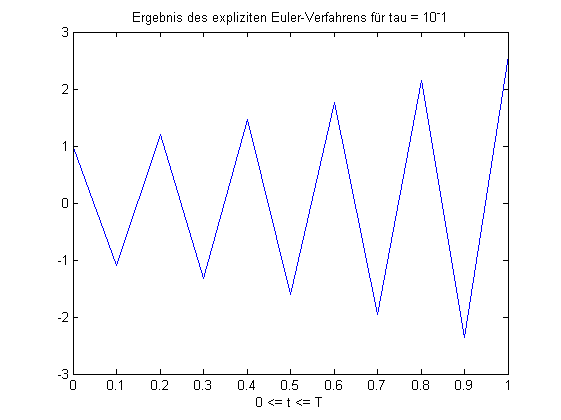
\includegraphics[scale=0.44]{exeuler1.png}
%}
%\subfigure[Plot des expliziten Euler-Verfahrens mit $\tau = 0.01$]{
%	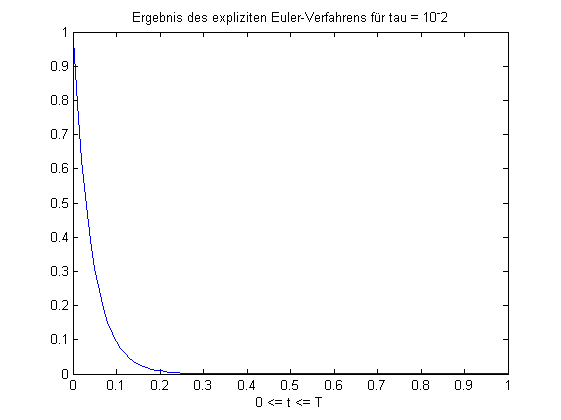
\includegraphics[scale=0.44]{exeuler2.png}
%}
%\subfigure[Plot des expliziten Euler-Verfahrens mit $\tau = 0.001$]{
%	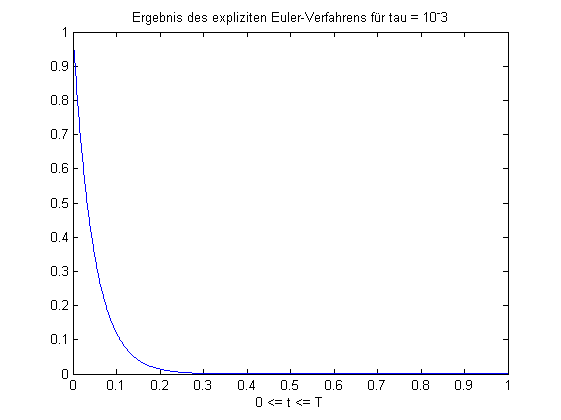
\includegraphics[scale=0.44]{exeuler3.png}
%}
%\end{figure}

\begin{description}
\item[a)] Sei nun $f(t) = 4\pi \cos(4\pi t) - \lambda \sin(4\pi t), \lambda = -1, x_0 = 1$ und $T = 2$ und die Schrittweite $\tau = T/100 = 0.02$. \\

(1) Exakte Lösung des AWP:
\begin{eqnarray*}
x(t) &=& e^{-t} + \int_0^t f(x) e^{-t+x} \; dx = e^{-t} + e^{-t} \int_0^t f(x)e^{x} \; dx
\end{eqnarray*}

Das Integral lösen wir nun durch partielle Integration, dazu bilden wir die ersten beiden Ableitungen von $f$, die wir in der partiellen Integration benutzen werden.
Dann gilt für die erste Ableitung $f'$:
\begin{eqnarray*}
f'(t) &=& (4\pi \cos(4\pi t) - \lambda \sin(4\pi t))' \\
&=& (4\pi \cos(4\pi t))' - (\lambda \sin(4\pi t))' \\
&=& (-16 \pi^2 \sin(4 \pi t)) - (4 \pi \lambda \cos(4 \pi t)) \\
&=& -16 \pi^2 \sin(4 \pi t) - 4 \pi \lambda \cos(4 \pi t)
\end{eqnarray*}
Und damit für die zweite Ableitung $f''$:
\begin{eqnarray*}
f''(t) &=& (-16 \pi^2 \sin(4 \pi t) - 4 \pi \lambda \cos(4 \pi t))' \\
&=& (-16 \pi^2 \sin(4 \pi t))' - (4 \pi \lambda \cos(4 \pi t))' \\
&=& (-16 \cdot 4 \pi^3 \cos(4 \pi t)) - (-16 \pi^2 \lambda \sin(4 \pi t)) \\
&=& -16 \cdot 4 \pi^3 \cos(4 \pi t) + 16 \pi^2 \lambda \sin(4 \pi t) \\
&=& -16 \pi^2 \left( 4 \pi \cos(4 \pi t) - \lambda \sin(4 \pi t)\right) \\
&=& -16 \pi^2 f(t)
\end{eqnarray*}
Nun können wir partiell integrieren:
\begin{eqnarray*}
\int_0^t f(x)e^{x} \; dx &=& [e^{x} \cdot f(x)]_0^t - \int_0^t e^{x} f'(x) \; dx \\
&=& [e^{x} \cdot f(x)]_0^t - \left([e^{x} \cdot f'(x)]_0^t - \int_0^t e^x f''(x) \; dx \right) \\
&=& [e^{x} \cdot f(x)]_0^t - [e^{x} \cdot f'(x)]_0^t + \int_0^t e^x f''(x) \; dx \\
&=& [e^{x} \cdot f(x)]_0^t - [e^{x} \cdot f'(x)]_0^t + \int_0^t e^x -16 \pi^2 f(x) \; dx \\
&=& [e^{x} \cdot f(x)]_0^t - [e^{x} \cdot f'(x)]_0^t - 16 \pi^2 \int_0^t e^x f(x) \; dx \\
\Rightarrow 17 \pi^2 \int_0^t f(x)e^{x} \; dx &=& [e^{x} \cdot f(x)]_0^t - [e^{x} \cdot f'(x)]_0^t \\
&=& (e^t \cdot f(t) -  e^0 \cdot f(0)) - (e^t \cdot f'(t) -  e^0 \cdot f'(0)) \\
%&=& e^t \cdot (4\pi \cos(4\pi t) - \lambda \sin(4\pi t)) -  e^0 \cdot (4\pi \cos(0) - \lambda \sin(0)) - e^t \cdot (-16 \pi^2 \sin(4 \pi t) - 4 \pi \lambda \cos(4 \pi t)) +  e^0 \cdot (-16 \pi^2 \sin(0) - 4 \pi \lambda \cos(0)) \\
&=& e^t \cdot (4\pi \cos(4\pi t) - \lambda \sin(4\pi t)) - 4 \pi \\
&-& e^t \cdot (-16 \pi^2 \sin(4 \pi t) - 4 \pi \lambda \cos(4 \pi t)) - 4\pi \lambda \\
&=& e^t 4\pi \cos(4\pi t) - e^t \lambda \sin(4\pi t) - 4\pi \\
&+& e^t 16 \pi^2 \sin(4 \pi t) + e^t 4 \pi \lambda \cos(4 \pi t) - 4\pi \lambda \\
&\stackrel{\lambda = -1}{=}& e^t 4\pi \cos(4\pi t) + e^t \sin(4 \pi t) - 4\pi \\\
&+& e^t 16 \pi^2 \sin(4 \pi t) - e^t 4 \pi \cos(4 \pi t) + 4 \pi \\
&=& e^t \sin(4 \pi t) + e^t 16 \pi^2 \sin(4 \pi t)
\end{eqnarray*}
irgendwo kleine lücke...glaub ich.
soll rauskommen: 
$x(t) = e^{-t} + \sin(4\pi t)$
also integral = $e^t * sin(4pi t)$
TODO!


(2) Approximative Lösung des AWP mit $\Theta = 0, 0.5, 1$. \\
tda

\item[b)]
\end{description}

%% ------------------------------------------------------
%%                     AUFGABE 3
%% ------------------------------------------------------

%%\section*{Aufgabe 3}


\label{LastPage}

\end{document}
